\documentclass[12pt,a4paper,oneside,titlepage]{article}
\usepackage[utf8]{inputenc}
\usepackage[english, russian]{babel}
\usepackage{amsmath}
\usepackage{amsfonts}
\usepackage{amssymb}
\usepackage{textcase} 
\usepackage{tocloft}
\usepackage{lastpage}
\usepackage{graphicx}
\usepackage[left=3.5cm,right=1cm,top=2cm,bottom=2cm]{geometry}
\author{Kostenko}
\setcounter{tocdepth}{3}%для глубины страницы содаржения
\renewcommand{\baselinestretch}{1.25}
\renewcommand{\cftsecleader}{\cftdotfill{\cftdotsep}} % точки в содержании для секций
\bibliographystyle{unsrt}
\begin{document}
{
\thispagestyle{empty}
\newpage
\centering

\textbf{
National Research University Higher School of Economics\\
}
Faculty of Business Informatics\\
School of Software Engineering\\
Software Management Department

\vfill


\begin{large}
\MakeTextUppercase{
An Application for Dynamic Object Identification Based on Lucas-Kanade Algorithm
}
\end{large}


\vfill

\begin{tabular}{lr}
Student: & Kostenko Dmitry \\
Group: & 472SE \\
Argument Consultant: & Prof. Ivan. M. Gostev, PhD \\
Style and Language Consultant: & Tatiana A. Stepantsova
\end{tabular}

\vspace{\fill}

Moscow\\ \number\year
\clearpage
}

\section*{Abstract}
{
В данной статье описывается подход к обнаружению и подсчету транспортных средств на атодорогах.
Он основан на дифференциальном методе вычисления оптического потока, предложенном Лукасом и Канаде.
Отличие данного метода от других состоит в том, что нет необходимости подготавливать модель фона.
}









{
\newpage
\centering
\tableofcontents
}











\newpage
\section*{Introduction}
\addcontentsline{toc}{section}{Introduction}
Nowadays it is possible to notice high grow of vehicles in all Russian cities.
According to DPS data annual growth of cars number is 110 - 120 thousand.
As a result the significance of traffic conjunction problem increases.
It causes higher fuel usage 
%Как следствие увеличивается расход топлива, уровень загрязнения окружающей среды и время пути каждого автомобилиста.
One of the decisions of the problem is installation of Intelligent Transportation System (ITS).
ITS ranges from simple traffic light control systems to systems which register velocity of vehicles flow, control traffic flow and recognition of the violations.

Such systems can perform the following tasks:

1) ensuring maximum traffic capacity;

2) reducing road accidents and monitoring human factor;

3) collecting information about traffic jams from the vehicle flow and informing its participants;

4) environment protection as a result of real-time monitoring of road situation and well timed decisions making.

ITS can contain various sensors from heat sensors to super-sound ones.
Manual processing of a significant amount of data which is received from the sensors is not applicable in the real-life situations.
As a consequence, a vital necessity of automation of the process and decision making, based the information gathered during this process, arises.

Automatic vehicle detection in this video monitoring is a complex objective of computer vision.

On of the tasks of such a system is to count vehicles on the highway.

In its turn, it is divided into subtasks of computer vision, such as foreground retrieving (vehicles) and tracking in the next frames.

This paper offers an overview of an approach which is related to automatic tracking of moving vehicles.
The only source of data used by this approach is a camera video recording.

The first chapter of the present graduation paper offers an overview of existing solution in the field of video monitoring.
Problem statement and requirements to the algorithm under development are covered in the second chapter.
The third chapter deals with description of methods and algorithms.
And finally, the brief exploration of expected results will be introduced.
%В наше время наблюдается высокие рост количества транспортных средств во всех городах России.
%По данным ГИБДД только в Москве ежегодный прирост автомобилей составляет 110 - 120 тысяч.
%В результате проблема заторов автотранспортных дорог становится более острой.
%Как следствие увеличивается расход топлива, уровень загрязнения окружающей среды и время пути каждого автомобилиста.
%Одним из решений данной проблемы является установка городской интелектуальной транспортной системы (ИТС).
%ИТС варьируются от простых систем регулирования светофоров, до систем регистрации скорости потоков транспортных средств, контроля автомобильного потока и распознования фактов нарушений.
%(http://ru.wikipedia.org/wiki/Интеллектуальная_транспортная_система)
%Такие системы позволяют решать следующие задачи.
%1) Обеспечение максимальной пропускной способности.
%1) Безопасность. Основная цель — снижение аварийности на дорогах. Сюда же входит мониторинг природных катаклихмов и человеческого фактора.
%2) Мобильность. Сбор информации о пробках от движущихся в потоке автомобилей и информирование участников движения.
%3) Защита окружающей среды. Снижение ущерба окружающей среде от автотранспорта посредством мониторинга ситуации в реальном времени и своевременного принятия решений.
%ИТС может содержать в себе датчики различных типов, от тепловых до ультразвуковых.
%Ручная обработка гигантского объема данных, поступающих от всех сенсоров таких систем непрактична.
%Поэтому появляется необходимость автоматизировать обработку данных и заключения выводов на основе них.
%Автоматическое обнаружение транспортных средств в данных видеонаблюдения является комплексной задача в компьютерном зрении.
%Одной из задач такой системы является подсчет транспортных средств на автодороге.
%Которая в свою очередь тоже разбивается на подзадачи компьютерного зрания, такие как: выделение объектов переднего плана (автомобилей) и отслеживание их положения в последующих кадрах.
%В данной статье мы описываем подход к решению задачи автоматического отслеживания движущихся транспортных средств и их подсчета.
%Где единственным источником данных о ситуации на автодороге является видеокамера. 
%Краткое содержание последующих глав:
%3) Обзор существующих решений в области видеонаблюдения на автодорогах.
%4) Постановка задачи и формулирование требований к разрабатываемому алгоритму.
%5) Изложение методов и алгоритмов решения поставленной задачи
%6) Краткое содержание планируемых рещультатов работы и выводы.

















\newpage
\section*{Related work}
\addcontentsline{toc}{section}{Related work}
В данной главе представлен краткий обзор существующих решений в области видеонаблюдения на автодорогах.

В мире существует только одна всеобъемлющая архитектура ИТС. Предложенная транспортным департаментом США инициатива, направленная на создание единого информационного пространства, объединяющего автомобили, дорожное оборудование, диспетчерские залы и центры обработки данных по всей стране. Данная транспортная система запатентована правительством США.
%(http://www.iteris.com/itsarch/documents/physical/physical.pdf)

В городе Москве в 2012 году начала свое действие ИТС.
% http://mskit.ru/news20/no117891/

Существуют аналоги, частично реализующие функционал ИТС США.






























\newpage
\section*{Problem statement}
\addcontentsline{toc}{section}{Problem statement}
Резальтатом данной главы будет являтся список требований к алгоритму.

Для формальности приведем некоторые определения.

Т.к. видео - это последовательность кадров, то в каждый момент времени мы имеем один кадр, называемый текущим.
Если кадр i - текущий кадр, то кадр (i-1) - предыдущий.

Объектами переденго плана будем считать любые движущиеся объекты (транспортные средства, деревья, люди).
Определение объекта, как движущегося, зависит от характеристик камеры и окружающей обстановки.
Поэтому движущимися объектами назовем те объекты, которые меняют свое положение на текущем кадре, относительно предыдущего кадра.

Движущийся объект перед камерой или движущиеся камера в неподвижной обстановке ведет к изменения изображения.
Изображение видимого движения объекта называется оптическим потоком.

Существует несколько методов вычисления оптического потока.
Лукас и Канаде предложили дифференциальный подход.
О нем будет рассказано позже.

Теперь перейдем к постановке задачи.

Одна из наиболее важных задач в видео наблюдении состоит из идентификации объекта интереса и отслеживание его траектории в последующих кадрах.
Эта задача может быть разбита на подзадачи.
Первое, необходимо обнаружить объекты интереса или объекты переднего плана.
Обнаружение объектов интереса подразумевает под собой отделение переднего плана от фона на изображении.
В нашем случае объектами переднего плана являются движущиеся объекты.
А объектами фона будем считать все остальные объекты.
После того, как мы это сделали мы получим бинарную карту движущихся объектов на изображении.

Далее необходимо понять, какие из движущихся объектов являются автотранспортными средствами, а какие не являются таковыми. 
Так как на изображении могут двигаться не только объекты переднего плана, но и объекты заднего плана (например ветви деревьев), то появляется необходимость борьбы с данным явлением.
Для этого ограничим на изображении область, в которой мы и будем вести видеонаблюдение. %рисунок
Такой областью лучше всего выделить хорошо просматриваемый промежуток автодороги.



О том, как выделять объект интереса (ограничевающей рамкой или попиксельной маской) будет написанно позже.

Затем следить за изменениями координат обектов интереса в последующих кадрах.





Для вычисления оптического потока необходимо сделать несколько предположений.

1) изображение - это непрерывная функция от двух переменных;
2) яркость объекта остается неизменной в небольшой промежуток времени;
3) отслеживаеммый объект на новом кадре будет расположен на небольшом расстоянии относительно предыдущего кадра.

Первое предположение дает нам возможность использовать методы математического анализа и позволяет производить матемстические операции над изображением.
Второе предположение существует потому, что мы живем в реальном мире, в котором  обхекты не могут мгновенно перемещаться на большие расстояния.
Третье предположение необходимо потому что мы не сможем без него отслеживать объект.




У данного подхода есть свои существунные недостатки.
Например, мы предпологаем, что камера является неподвижной.
Хотя в реальных условиях камера может быть подвержена движению, от порывов ветра.
Или на объектив камеры могут попадать капельки дождя, которые могут быть зафиксированы, как объекты переднего плана.





Сформулируем требования к алгоритму:
1) Работать без каких-либо предварительных данных об автодороге
2) Обработка потока данных в реальном времени
3) Не должен требовать высоких вычислительных мощностей. Минимальные требования к оборужованию будут предложены в техническом задании.
































\newpage
\section*{Algorithm}
\addcontentsline{toc}{section}{Algorithm}

In the following chapter an approach to the task of vehicles on motor ways detection and counting will be revealed.

As a video is a frame sequence, at every moment only one frame is available.

In the beginning, it is necessary to eliminate a noise of each frame.
Gauss filter must be applied in order to perform this.

The information about object color seems to be not in use in further.
Therefore it will be appropriate to transform the image from RGB color space to grayscale.
%В данной главе раскрывается подход к обнаружению и подсчету транспортных средств на атодорогах.
%Т.к. видео - это последовательность кадров, то в каждый момент времени мы имеем одно изображение.
%При получении нового кадра, сперва необходимо избавиться от шумов.
%Для этого сгладим изображение фильтром Гаусса. %ссылка на гауса

%Так как в дальнейшем мы не будем использовать информацию о цвете объектов, то для уменьшения количества избыточной информации переведем изображение из цветовой модели RGB в градации серого. %сказать каким алгоритмом

ПОСЛЕ УМЕНЬШИМ ИЗОБРАЖЕНИЕ





























\newpage
\section*{Allocation of foreground objects}
\addcontentsline{toc}{section}{Allocation of foreground objects}
The primary goal of the method, described in this section, is retrieving the foreground objects location.
%Целью метода, описанного в данном блоке, является получение положений объектов, относящихся к переднему плану.

The traditional algorithms of retrieving the foreground objects location are based on pixel-by-pixel frame difference method.
But this method also has several disadvantages.

\begin{figure}[h]
  \center{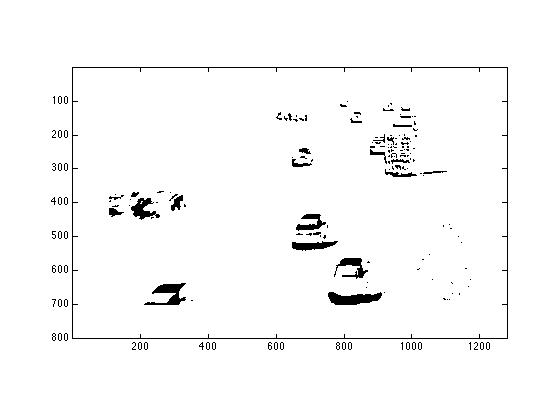
\includegraphics[width=10cm]{images/1.jpg}}
  \caption{Some caption}
  \label{fig:fig1}
\end{figure}


This method's application might lead to the  enormous amount of isolated areas.
For this reason, this method must be modified to avoid this disadvantage and to make these areas connected with each other.
At first, each frame has to be divided into blocks which do not overlap.
The optimal size of a block is found empirically and depends on characteristics of the camera and the environment.
That is why in the beginning the standard size will be assigned to each block - 3x3 pixels.

\begin{figure}[h]
  \center{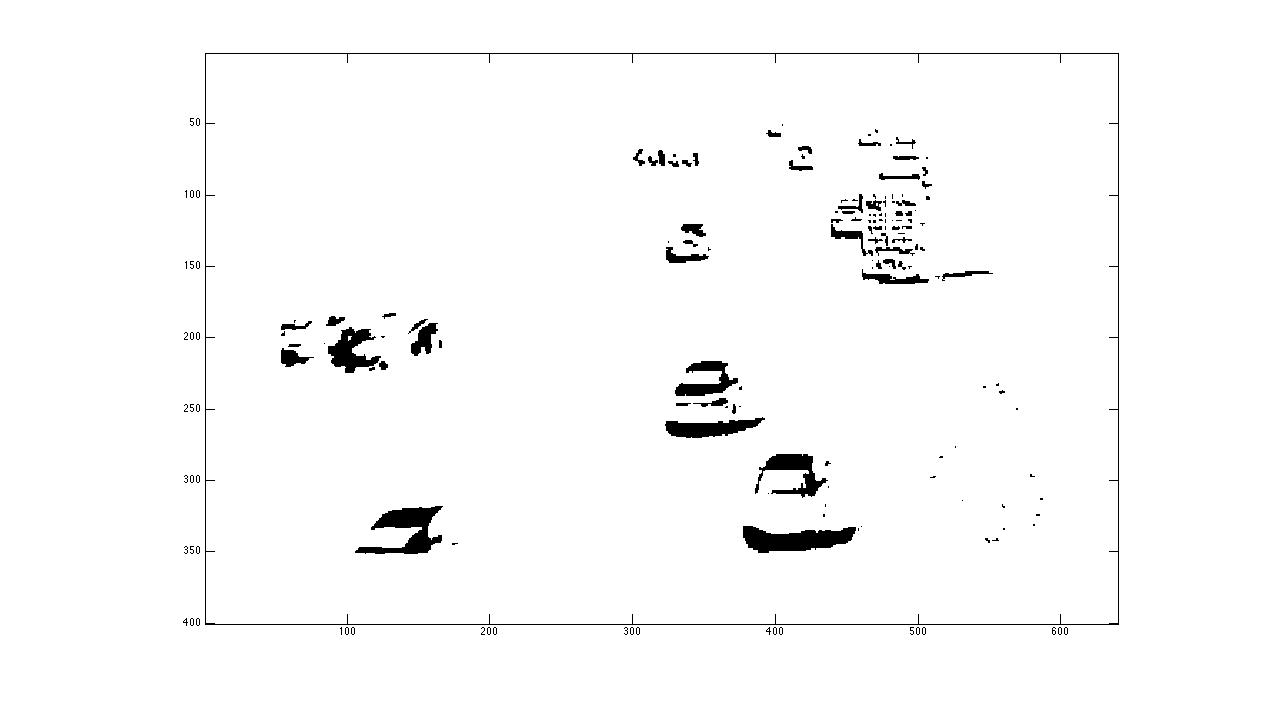
\includegraphics[width=10cm]{images/2.jpg}}
  \caption{Some caption}
  \label{fig:fig2}
\end{figure}



After that the previous frame is subtracted from the current frame.
Then every pixel block of the result is filtered in the following way:
if the amount of foreground objects pixels in every block is more than some pre-defined threshold, this block is considered to be the foreground
otherwise, it is concidered to be the background

As a result we get the binary image of the foreground objects.
But this image is not going to be perfect, it will definately have noise.
For that reason the image must be processed using morphological operations.
These operations are the following: erosion and dilation.

It is nesessary to consider that the method of subtracting the previous frame from the currrent frame gives good response near the moving object border. 
However, inside the objects borders the response is NOT SO GOOD.
If the vehicle is relatively large, the probability of its recognition as an object of the foreground is LITTLE.

To get rid of this effect let us consider two definitions: sort-term model of the foreground and long-term model of the foreground.


%Традиционные алгоритмы получения объектов переднего плана основаны на методе попиксельного вычитания изображений.
%Но у данного метода есть недостаток.
%С помощью него мы можем получить большое количество несвязных областей. %показать картинку

%Поэтому, для получения более связных областей, необходимо модифицировать данный метод.
%Сперва разобьем каждый кадр на непересекающиеся блоки.
%Оптимальный размер блока определяется империческии и зависит от характеристи камеры и окружающей обстановки.
%Поэтому, для начала, зададим размер блока равный 3х3 пикселей.
%Затем попиксельно вычтем предыдущий кадр из текущего.

%В конце, отфильтруем пиксели каждого блока у полученной разности изображений таким образом:
%если количество пикселей в каждом блоке, относящихся к объектам переднего плана, превышает заданный порог, то будем считать, что блок принадлежит переднему плану.
%В инном случаем будем считать обратное.

%В результате мы получим бинарное изображение объектов переднего плана.%показать картинку
%Но на данном изображении могут присутствовать шумы.
%Поэтому необходимо обработать изображение морфологическими операциями.
%Применим эррозию, а затем наращивание. % dilation



%Так же необходимо заметить, что метод вычитания предыдущего кадра из текущего дает хороший отклик на границе движущегося объекта.
%Но в оласти движущегося объекта наблюдается обратный эффект. %показать картинку
%В случае, когда транспортное средство имеет большие размеры, вероятность определить транспортное средство, как объект переднего плана, существенно уменьшается.

%Чтобы избежать подобного эффекта введем еще 2 понятия: краткосрочная модель переднего плана и долгострочная модель  переднего плана.

The short-term model is the model which we get, after applying the steps stated above.
The long-term model is the pixel-by-pixel sum of N previous short-term foreground models, where N is NATURAL and more than 1.  
N is found empirically and depends on characteristics of the camera and the environment.

As the objects that we want to track are moving, calculating the long-term model of  the foreground we get the object regions, which is more connected.

As can be seen from FIGURE 1 the object region can be separated into several regions.
To reduce the amount of these regions we use the dilation operation with pre-defined window.
%Краткосрочной моделью переднего плана является такая модель, которая получается в результате применения последовательности действий, описанных выше.
%Долгосрочной моделью переднего плана назовем попиксельную сумму N моедлей переднего плана, где N - натуральное число и больше 1.
%N зависит от характеристик камеры и окружающей среды вычисляется империческим путем.

%Т.к. отслеживаемые объекты движутся, то при вычислении долгосрочной модели переднего плана мы получим более свзные области предполагаемых транспортных средств. % показать кратинку
%На изображении видно, что область объекта может разделиться на несколько областей.
%Для уменьшения количества связных областей применим морфологическую операцию наращивание.






































\newpage
\section*{Foreground segmentation}
\addcontentsline{toc}{section}{Foreground segmentation}
В данной главе излагается метод сегментации объектов переднего плана.





Приведем содержание алгоритма, затем опишем каждый пункт.

1) Перевести изображение в серое
2) обработать изображение фильтром гауса (против шумов)
3) вычесть из текущего изображения предыдущее
4) наложить друг на друга n предыдущих разностей (для получения транспортного средства) Делать это каждые 5 кадров
5) выделить связные области, которые и будут предположительно транспортными средствами 
6) сопоставить текущия связные области с такими же на предыыдущих кадрах или инициализировать новые
7) если такая связна область пересекает линию интереса, то прибавляем 1 к счетчику



\newpage
\section*{Conclusion}
\addcontentsline{toc}{section}{Conclusion}
1 page


\newpage
\renewcommand\refname{Bibliography}
\bibliographystyle{plain}
\bibliography{draft}



\end{document}
